\subsection{Dominating Eigenvectors of Layer-wise Hessian are Low Rank}
\label{sec:appendix_low_rank_eigenvector}
% The structure of Hessians' eigenvectors is also important for assessing Hessian properties. 

A natural corollary for the Kronecker factorization approximation of layer-wise Hessians is that the eigenvectors of the layer-wise Hessians are low rank. Let $\vh_i$ be the $i$-th eigenvector of a layer-wise Hessian.
The rank of $\Mat(\vh_i)$ can be considered as an indicator of the complexity of the eigenvector. Consider the case that $\vh_i$ is one of the top eigenvectors. From \sectionref{sec:models}, we have $\vh_i \approx \vu_i \otimes \hE[\vx]$. % for some $\vu_i \in \R^m$.
Thus, $\Mat(\vh_i) \approx \vu_i\hE[\vx]^\T$, which is approximately rank 1. Experiments shows that first singular values of $\Mat(\vh_i)$ divided by its Frobenius Norm are usually much larger than 0.5, indicating the top eigenvectors of the layer-wise Hessians are very close to rank 1.
\figureref{fig:eigen_lowrank} shows first singular values of $\Mat(\vh_i)$ divided by its Frobenius Norm for $i$ from 1 to 200. We can see that the top eigenvectors of the layer-wise Hessians are very close to rank 1.
 \begin{figure}[h]
     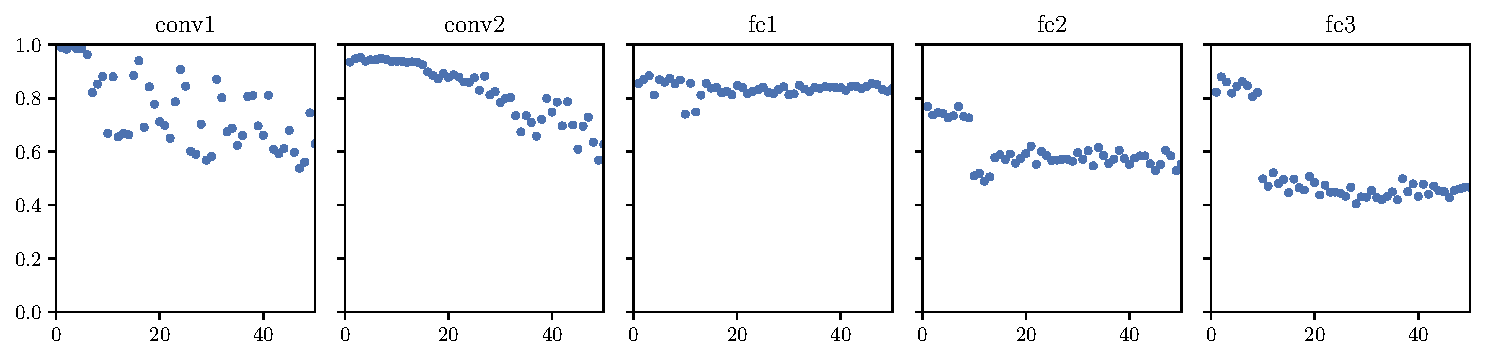
\includegraphics[width=\columnwidth]{Figures/Eigenvec_Lowrank/NLeNet_base/5x1_Top_Eigenvector_rank_CIFAR10_Exp1_LeNet5_normnew_fixlr0.01R2_E-1_50.pdf}
    %  \captionsetup{justification=centering}
      \vspace{-0.2in}
     \caption{Ratio between top singular value and Frobenius norm of matricized dominating eigenvectors. (LeNet5 on CIFAR10). The horizontal axes denote the index $i$ of eigenvector $\vh_i$, and the vertical axes denote $\|\Mat(\vh_i)\|/\|\Mat(\vh_i)\|_F$.}
    \label{fig:eigen_lowrank}
     \vspace{-2em}
 \end{figure}